\chapter{Limitaciones del modelo clásico}
\label{ch:limitaciones}

El modelo de Markowitz formulado en el Capítulo~\ref{ch:formulacion} es
matemáticamente impecable: dado un vector de rentabilidades esperadas
$\boldsymbol{\mu}$ y una matriz de covarianza $\boldsymbol{\Sigma}$, el
QP convexo produce la cartera óptima. Sin embargo, en la práctica
$\boldsymbol{\mu}$ y $\boldsymbol{\Sigma}$ no se conocen: deben
estimarse a partir de datos históricos. Este capítulo analiza las
consecuencias del error de estimación, presenta dos enfoques para
mejorar la estimación de $\boldsymbol{\Sigma}$ (shrinkage de Ledoit-Wolf
y modelos de factores basados en PCA) y motiva el uso de Machine Learning para estimar
$\boldsymbol{\mu}$.

%--------------------------------------------------------------------
\section{El error de estimación y sus consecuencias}
%--------------------------------------------------------------------

\subsection{Dimensionalidad y escasez de datos}

El modelo de Markowitz requiere estimar $n$ rentabilidades esperadas y
$n(n+1)/2$ covarianzas distintas. Para nuestro universo de $n = 30$
activos, esto supone $30 + 30 \times 31 / 2 = 495$ parámetros. Con una
ventana de estimación de 3 años de datos mensuales ($T = 36$
observaciones), el cociente $n/T \approx 0{,}83$ es demasiado alto: los
495 parámetros se estiman con solo $30 \times 36 = 1080$ datos, poco más
de dos datos por parámetro.

En estas condiciones, el estimador muestral de $\boldsymbol{\Sigma}$,
aunque insesgado, tiene una varianza muy elevada. Los autovalores
pequeños de la matriz muestral están sistemáticamente infraestimados
y los grandes, sobreestimados \cite{Ledoit2004}. Esto tiene
consecuencias directas sobre la optimización: el QP explota estos
errores, asignando pesos desproporcionados a activos cuya covarianza
está mal estimada.

\subsection{El problema de la estimación de \texorpdfstring{$\boldsymbol{\mu}$}{μ}}

Si estimar $\boldsymbol{\Sigma}$ es difícil, estimar $\boldsymbol{\mu}$
lo es aún más. La rentabilidad esperada de un activo es muy
ruidosa: la desviación típica de la media muestral es
$\sigma / \sqrt{T}$, que con $\sigma \approx 0{,}05$ mensual y
$T = 36$ meses da aproximadamente $0{,}0083$, comparable a la propia
media muestral para muchos activos. En otras palabras, la incertidumbre
en la estimación de $\boldsymbol{\mu}$ es del mismo orden de magnitud
que el propio parámetro.

Merton \cite{Merton1980} demostró que, mientras la varianza puede
estimarse con precisión creciente al aumentar la frecuencia de
observación, la precisión de la estimación de la media depende
únicamente del horizonte temporal total, no de la frecuencia. Con 15
años de datos, la media anualizada tiene un error estándar de
$\sigma_{\text{anual}}/\sqrt{15} = 0{,}05\cdot\sqrt{12}/\sqrt{15}
\approx 0{,}045$: unos 4,5 puntos porcentuales de incertidumbre, del
mismo orden que la propia rentabilidad que se quiere estimar.

Este es el punto débil que el Machine Learning puede
ayudar a mitigar: si existe una relación predecible entre las
características observables de los activos y sus rentabilidades
futuras, un modelo predictivo puede producir una estimación de
$\boldsymbol{\mu}$ más precisa que la simple media histórica
(Capítulo~\ref{ch:ml}).

%--------------------------------------------------------------------
\section{Inestabilidad y concentración de los pesos}
%--------------------------------------------------------------------

\subsection{Demostración empírica}

Para ilustrar el problema, comparamos las carteras de mínima varianza
(GMV) obtenidas con tres estimadores de $\boldsymbol{\Sigma}$ sobre la
misma ventana de 3 años (enero 2022 -- diciembre 2024). Se usa la GMV porque no
depende de las rentabilidades esperadas $\boldsymbol{\mu}$, sino solo de la
covarianza $\boldsymbol{\Sigma}$; así, cualquier diferencia entre las tres
carteras se debe únicamente al estimador de $\boldsymbol{\Sigma}$. La
Tabla~\ref{tab:comparativa-sigma} resume los resultados.

\begin{table}[htbp]
    \centering
    \caption{Comparación de carteras GMV según el estimador de
             $\boldsymbol{\Sigma}$. Ventana: 2022--2024 (36 meses).}
    \label{tab:comparativa-sigma}
    \begin{tabular}{lccc}
\toprule
Estimador & Activos $>$ 1\% & HHI & $\sigma_p$ (mensual) \\
\midrule
Muestral & 10 & 0.137 & 3.25\% \\
Ledoit-Wolf & 14 & 0.099 & 3.12\% \\
PCA (80\%) & 11 & 0.130 & 3.28\% \\
\bottomrule
\end{tabular}

\end{table}

El estimador muestral concentra la cartera en solo 10 activos (de 30)
con un índice Herfindahl-Hirschman (HHI) de $0{,}137$. El HHI se define
como:
\begin{equation}
    \text{HHI} = \sum_{i=1}^{n} w_i^2,
    \label{eq:hhi}
\end{equation}
y toma el valor $1/n \approx 0{,}033$ para la cartera equiponderada
(máxima diversificación) y $1$ para una cartera concentrada en un solo
activo.

El estimador de Ledoit-Wolf aumenta la diversificación a 14 activos
y reduce el HHI a $0{,}099$, mientras que el estimador PCA se sitúa en
una posición intermedia (11 activos, HHI $0{,}130$). La volatilidad
es muy similar en los tres casos (3,12\%--3,28\% mensual), lo que
sugiere que las diferencias en los pesos no se traducen necesariamente
en diferencias grandes de riesgo ex-ante (el riesgo estimado antes de invertir),
pero sí pueden afectar la estabilidad temporal y el turnover.

\subsection{Evolución temporal de la concentración}

La Figura~\ref{fig:hhi-temporal} muestra la evolución del HHI a lo
largo del tiempo utilizando ventanas móviles de 3 años (una ventana de 36 meses
que avanza mes a mes). Se observa
que el estimador muestral (azul) produce carteras sistemáticamente
más concentradas y con mayor variabilidad en el nivel de concentración
a lo largo del tiempo. El estimador de Ledoit-Wolf (naranja) mantiene
un HHI siempre más bajo y más estable, mientras que el
estimador PCA (verde) presenta un comportamiento intermedio.

\begin{figure}[htbp]
    \centering
    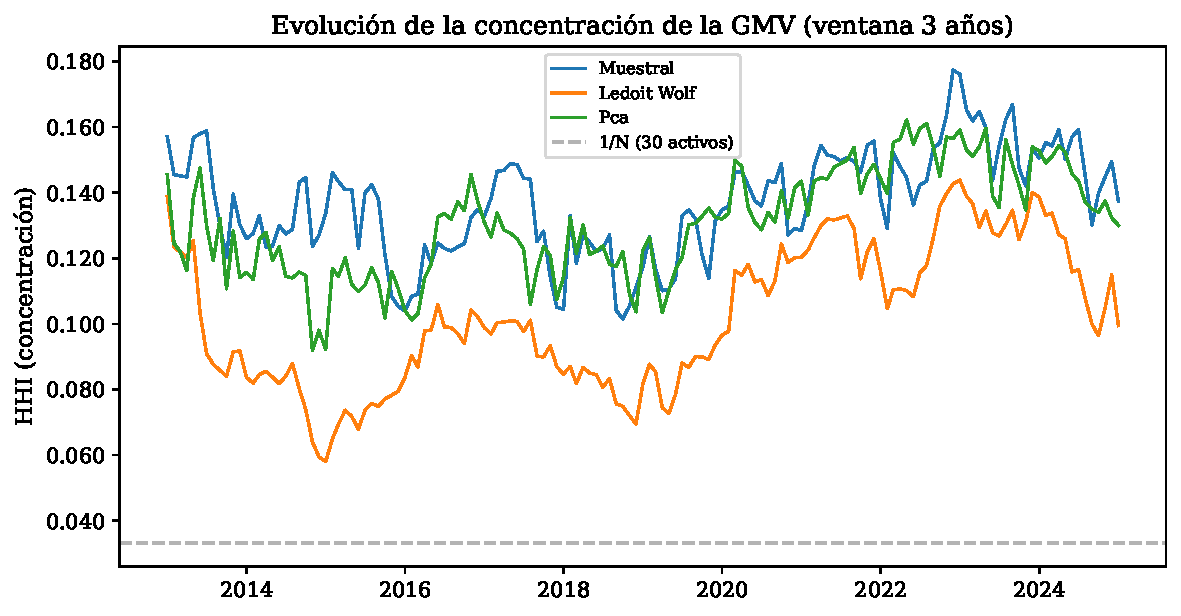
\includegraphics[width=0.60\textwidth]{../data/outputs/hhi_temporal}
    \caption{Evolución del índice Herfindahl-Hirschman (HHI) de la
             cartera GMV con ventanas móviles de 36 meses. La línea
             gris discontinua marca el HHI de la cartera equiponderada
             ($1/30 \approx 0{,}033$).}
    \label{fig:hhi-temporal}
\end{figure}

La inestabilidad de los pesos provoca dos problemas. El primero es un
\textbf{turnover} elevado: si los pesos óptimos cambian mucho de un mes a otro,
hay que comprar y vender activos con frecuencia, y esas comisiones reducen la
rentabilidad final. El segundo es la \textbf{concentración}: la cartera acaba
invertida en pocos activos, justo lo contrario de diversificar, y así asume el
riesgo particular de esos títulos, un riesgo que el mercado no remunera porque
podría haberse eliminado repartiendo mejor la inversión.

%--------------------------------------------------------------------
\section{Estimación robusta de la covarianza: shrinkage de Ledoit-Wolf}
\label{sec:ledoit-wolf}
%--------------------------------------------------------------------

\subsection{Fundamento teórico}

La idea del \textit{shrinkage} es sencilla: en lugar de fiarse por completo de
la matriz muestral (precisa en promedio, pero muy ruidosa), se mezcla con una
matriz simple y estable, y se toma un punto intermedio. Formalmente, el
\textit{shrinkage} es una técnica de regularización que contrae el estimador
muestral hacia un estimador estructurado (el \textit{target}), reduciendo el
error cuadrático medio esperado a cambio de introducir un pequeño sesgo. Ledoit
y Wolf \cite{Ledoit2004} propusieron un estimador de covarianza que es
combinación convexa (una media ponderada) del estimador muestral
$\boldsymbol{\Sigma}_{\text{muestral}}$ y un target
$\boldsymbol{\Sigma}_{\text{target}}$:
\begin{equation}
    \boldsymbol{\Sigma}_{\text{LW}} = (1 - \delta)\,
    \boldsymbol{\Sigma}_{\text{muestral}} + \delta\,
    \boldsymbol{\Sigma}_{\text{target}},
    \label{eq:ledoit-wolf}
\end{equation}
donde $\delta \in [0, 1]$ es la intensidad de shrinkage, calculada
analíticamente para minimizar el error cuadrático medio esperado
asintóticamente.

El target por defecto en \texttt{scikit-learn} (y en nuestra implementación) es
una \textbf{identidad escalada}: una matriz diagonal cuyos elementos valen todos
la varianza media de los activos, con correlaciones nulas fuera de la diagonal,
\begin{equation}
    [\boldsymbol{\Sigma}_{\text{target}}]_{ij} =
    \begin{cases}
        \bar{\sigma}^2 & \text{si } i = j, \\
        0 & \text{si } i \neq j,
    \end{cases}
    \qquad
    \bar{\sigma}^2 = \frac{1}{n}\sum_{k=1}^{n} \sigma_{kk}^{\text{muestral}}.
    \label{eq:target-lw}
\end{equation}
Es un target muy bien condicionado (todos sus autovalores valen
$\bar{\sigma}^2$), y al mezclarlo con la matriz muestral se atenúan los
autovalores extremos y las correlaciones espurias.

\subsection{Efecto sobre la cartera}

El efecto del shrinkage sobre los pesos de la cartera GMV se aprecia
en la Tabla~\ref{tab:comparativa-sigma}: la cartera Ledoit-Wolf es la
más diversificada de las tres. Esto se debe a que el shrinkage contrae
los autovalores hacia su media: baja los más grandes y, sobre todo, sube
los más pequeños, que son los que hacen inestable a
$\boldsymbol{\Sigma}^{-1}$ y los que el QP explotaría para concentrar
los pesos.

La Figura~\ref{fig:pesos-estimadores} compara visualmente la
distribución de pesos obtenida con cada estimador.

\begin{figure}[htbp]
    \centering
    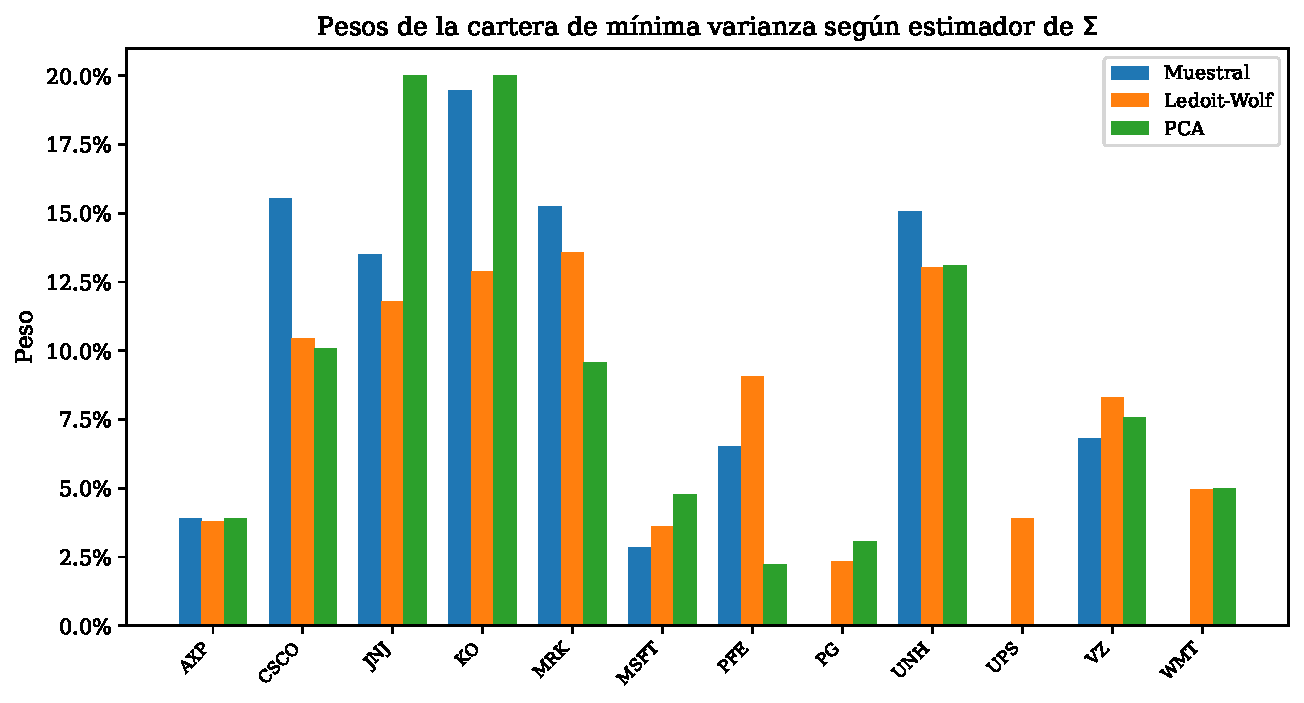
\includegraphics[width=0.66\textwidth]{../data/outputs/pesos_por_estimador}
    \caption{Pesos de la cartera GMV según el estimador de
             $\boldsymbol{\Sigma}$ (solo activos con peso $> 2\%$
             en al menos un estimador).}
    \label{fig:pesos-estimadores}
\end{figure}

%--------------------------------------------------------------------
\section{Covarianza basada en PCA y modelos de factores}
\label{sec:pca}
%--------------------------------------------------------------------

La idea es que casi todo lo que mueve a los activos a la vez se debe a unos
pocos factores comunes, como el mercado en su conjunto o los sectores; el PCA
identifica esos factores y separa esa estructura común del ruido propio de cada
activo. La matriz de covarianza muestral admite una descomposición espectral
$\boldsymbol{\Sigma} = \sum_{i=1}^{n} \lambda_i \mathbf{v}_i \mathbf{v}_i^T$,
con autovalores $\lambda_1 \ge \dots \ge \lambda_n \ge 0$, cada uno la varianza
explicada por su componente principal. El estimador PCA retiene solo los $k$
primeros componentes (los factores comunes), descarta el resto como ruido y
conserva la varianza específica de cada activo; su construcción detallada se
recoge en el Apéndice~\ref{ap:pca-apt}.

\subsection{Selección del número de factores}

La Figura~\ref{fig:scree-plot} muestra los autovalores de la matriz
de covarianza muestral y la varianza explicada acumulada para la
ventana 2022--2024.

\begin{figure}[htbp]
    \centering
    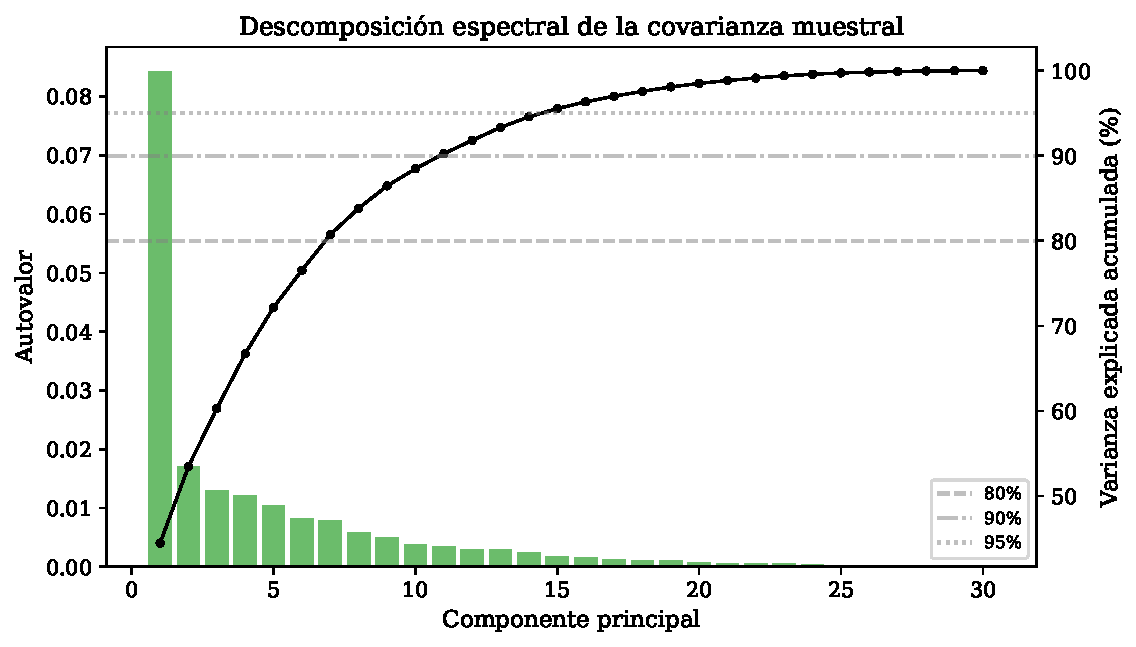
\includegraphics[width=0.55\textwidth]{../data/outputs/scree_plot}
    \caption{Descomposición espectral de la covarianza muestral.
             Barras: autovalores (eje izquierdo). Línea: varianza
             explicada acumulada (eje derecho).}
    \label{fig:scree-plot}
\end{figure}

El primer componente principal explica el 44,5\% de la varianza total;
con 7 componentes se alcanza el 80\% y con 11 componentes el 90\%.
Esto indica que la mayor parte de la variabilidad de las rentabilidades
de los 30 activos puede capturarse con un número reducido de factores
comunes, lo que justifica el uso de un modelo de factores para la
estimación de la covarianza.

\subsection{Conexión con la Arbitrage Pricing Theory (APT)}

La \textit{Arbitrage Pricing Theory} (APT) de Ross \cite{Ross1976} sostiene que
las rentabilidades de los activos dependen de unos pocos factores de riesgo
comunes y de una parte propia de cada activo. La conexión con lo anterior es
directa: si se toman como factores los $k$ primeros componentes principales, el
estimador PCA coincide exactamente con ese modelo de factores (la equivalencia
se demuestra en el Apéndice~\ref{ap:pca-apt}). Dicho de otro modo, los
componentes principales de la covarianza actúan como los factores de riesgo de
la teoría financiera. Esta correspondencia conecta el enfoque puramente
estadístico (la descomposición espectral) con la teoría financiera de factores,
y es uno de los puntos metodológicamente más relevantes de este trabajo.

%--------------------------------------------------------------------
\section{Síntesis: del error de estimación a la necesidad de Machine Learning}
%--------------------------------------------------------------------

La estimación de $\boldsymbol{\Sigma}$ puede mejorarse con regularización
(shrinkage) o reducción de dimensionalidad (PCA), pero la de
$\boldsymbol{\mu}$ sigue siendo el punto débil del modelo. De hecho, la
Tabla~\ref{tab:comparativa-sigma} muestra que los tres estimadores de
$\boldsymbol{\Sigma}$ dan volatilidades muy parecidas con pesos muy distintos:
la elección del estimador afecta más a la composición de la cartera que a su
riesgo ex-ante. La rentabilidad realizada, en cambio, depende sobre todo de
$\boldsymbol{\mu}$, el parámetro más difícil de estimar. De ahí que el
Capítulo~\ref{ch:ml} recurra al Machine Learning para predecirlo: si se estima
mejor $\boldsymbol{\mu}$, se puede aspirar a carteras con rentabilidad
out-of-sample superior a las estrategias pasivas de referencia.
